\documentclass[presentation]{beamer}
\usepackage{../oop-slides-pianini}
\setbeamertemplate{bibliography item}[text]
\title[OOP03 -- Interfaces]{03\\Eclipse IDE, Incapsulamento e Interfacce}
\author[Pianini]{Danilo Pianini\\Giovanni Ciatto, Angelo Croatti, Mirko Viroli}

\begin{document}
	
\frame[label=coverpage]{\titlepage}

\begin{frame}<beamer>
	\frametitle{Outline}
	\tableofcontents[]
\end{frame}

\section{Eclipse IDE}
\subsection{Introduzione}

\begin{frame}{Integrated Development Environment (IDE)}
	\begin{block}{}
		\emph{A software suite that consolidates the basic tools developers need to write and test software. An IDE contains a code editor, a compiler and a debugger that the developer accesses through a single user interface.}
	\end{block}
	\begin{itemize}
		\item Ambiente integrato per la creazione e la gestione di progetti software.
		\begin{itemize}
			\item Un progetto, per un IDE, è composto da una collezione organizzata di risorse: sorgenti, librerie, compilati, documentazione, \dots
		\end{itemize}
		\item Componenti tipici di un IDE:
		\begin{itemize}
			\item Editor di testo con syntax highlighting (e code completion)
			\item Compilatore
			\item Macchina(e) virtuale per l'esecuzione e il debugging delle applicazioni
			\item Strumenti per agevolare il deployment (distribuzione) delle applicazioni
		\end{itemize}
		\item Esempi di IDE:
		\begin{itemize}
			\item Eclipse, NetBeans, IntelliJ IDEA, Microsoft Visual Studio, XCode, \dots
		\end{itemize}
	\end{itemize}
\end{frame}

\begin{frame}{Diffusione dei principali IDE}
	\begin{center}
		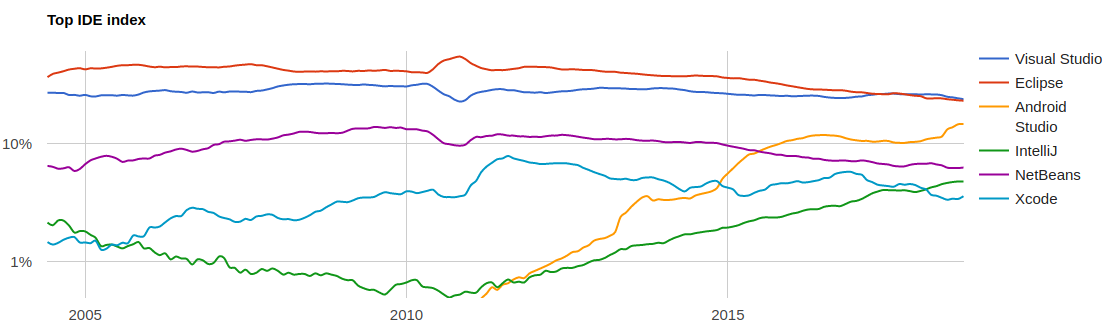
\includegraphics[width=\textwidth]{img/ide2018.png}
	\end{center}
	\centering
	Dati da \url{https://pypl.github.io/IDE.html}
\end{frame}



\fr{Eclipse Overview}{
	\bl{Overview}{
		\iz{
			\item Eclipse è un IDE open-source scritto in Java 
			\item Disponibile per diverse piattaforme (Windows, Linux, Mac OSX, ..)
			\item 	.. e sotto forma di diverse distribuzioni 
				\iz{
					\item	Standard, per sviluppatori J2EE/C/C++/Python/Web.. 
				}
			}
	}
	\bl{Un po' di storia}{
		\iz{
			\item Nato nei laboratori di ricerca IBM (alphaWorks) 
			\item	Successivamente	donato alla comunità open-source che ora ne cura lo sviluppo per mezzo di un'apposita fondazione
			\item Correntemente supportato/utilizzato da un vasto numero di sviluppatori, sia in ambito accademico che industriale
		}
	}
}

\begin{frame}[allowframebreaks]{Astrazioni di base}
	\begin{block}{Workspace}
		Directory dove Eclipse salva e carica le impostazioni di un certo numero di progetti. Tipicamente contiene anche i progetti (che possono però anche essere importati da altre directory)
	\end{block}
	\begin{block}{Progetto}
		Directory contenente una collezione di risorse opportunamente organizzate, tipicamente rappresentanti un software o una parte di un software
	\end{block}
	\begin{block}{Plug-in}
		Software installabile opzionalmente che estende le capacità dell'IDE, ad esempio:
		\begin{itemize}
			\item controllare la qualità del codice Java;
			\item aggiungere supporto ad ulteriori linguaggi;
			\item usare sistemi di build diversi da quello predefinito (Gradle, Maven...);
		\end{itemize}
	\end{block}
	\begin{block}{View}
		Componente dell'interfaccia di Eclipse.
		\begin{itemize}
			\item Tipicamente numerose view sono aperte contemporaneamente;
			\item Ciascuna offre una micro-funzionalità, ad esempio:
			\begin{itemize}
				\item Package Explorer --- fornisce una vista dei progetti e della loro struttura;
				\item Console --- consente di usare un terminale interno all'IDE invece del terminale di sistema;
				\item Outline --- mostra un riassunto dei componenti della classe attualmente aperta, elencando i membri, consentendo di filtrarli (ad esempio, nascondendo i privati) e di ordinarli (ad esempio in ordine alfabetico);
				\item Problems --- elenca gli eventuali problemi che affliggono il progetto (errori 
di configurazione, sorgenti che non compilano, warnings...)
			\end{itemize}
		\end{itemize}
	\end{block}
	\begin{block}{Perspective}
		Insieme di view che vengono. Cambiare perspective consente di cambiare rapidamente le view attive. Tipicamente, si usano perspective diverse per fasi diverse dello sviluppo. Ne vedremo sicuramente due:
		\begin{itemize}
			\item Java --- per lo sviluppo di applicazioni Java
			\item Debug --- per il debug di applicazioni (prossima lezione!)
		\end{itemize}
	\end{block}
\end{frame}


\subsection{Avvio e creazione di progetti}

\fr{Avvio di Eclipse: Scelta del Workspace}{
	\fg{width=\textwidth}{img/eclipse_startup.png}	
}
\fr{Creazione di Progetti Java 1/3}{
	\fg{height=0.85\textheight}{img/new_prj1.png}
}

\fr{Creazione di Progetti Java 2/3}{
	\fg{height=0.85\textheight}{img/new_prj2.png}
}

\fr{Creazione di Progetti Java 3/3}{
	\fg{height=0.85\textheight}{img/new_prj3.png}
}

\fr{Compilazione dei Sorgenti}{
	\fg{height=0.3\textheight}{img/eclipse_build.png}
	\bl{Due diverse possibilità}{
		\iz{
			\item Compilazione automatica
			\iz{
				\item Il compilatore viene invocato automaticamente dall'IDE ad ogni modifica (salvata) ai sorgenti del progetto
			}
			\item Compilazione manuale
			\iz{
				\item Attiva quando è disabilitata la compilazione automatica
				\item Il compilatore viene invocato a seguito di un esplicito click dello sviluppatore su \textit{``Build All''}
			}
		}
	}
}

\fr{Creazione di un Package 1/2}{
	\fg{height=0.8\textheight}{img/new_package1.png}
}

\fr{Creazione di un Package 2/2}{
	\fg{height=0.8\textheight}{img/new_package2.png}
}

\fr{Creazione di una Classe 1/2}{
	\fg{height=0.8\textheight}{img/new_class1.png}
}

\fr{Creazione di una Classe 2/2}{
	\fg{height=0.8\textheight}{img/new_class2.png}
}

\fr{JDT: Code Completion e Syntax Highlighting}{
	\fg{height=0.8\textheight}{img/sh_cc.png}
}

\fr{Esecuzione di Applicazioni}{
	\fg{height=0.8\textheight}{img/run1.png}
}

\fr{Esecuzione di Applicazioni: Un Alternativa 1/2}{
	\fg{height=0.8\textheight}{img/run2.png}
}

\fr{Esecuzione di Applicazioni: Un Alternativa 2/2}{
	\fg{height=0.8\textheight}{img/run3.png}
}

\fr{Esecuzione di Applicazioni: Output}{
	\fg{height=0.8\textheight}{img/run4.png}
}

\fr{Importazione di Progetti 1/2}{
	\fg{height=0.8\textheight}{img/import_prj1.png}
}

\fr{Importazione di Progetti Esistenti 2/2}{
	\fg{height=0.8\textheight}{img/import_prj2.png}
}

\subsection{Eclipse: Maggiori Dettagli}

\fr{Eclipse Architecture}{
	
	\bl{Eclipse ha una architettura organizzata a plug-in}{
		\iz{
			\item Un plug-in è un modulo (classi + meta-informazioni + manifest file) auto-contenuto che incapsula una certa funzionalità
				\iz{
						\item File editor specifici, wizard, build, compilazione e debugging di sorgenti
						\item Costituisce l'unità funzionale elementare dell'architettura
				}
			\item Possono essere definite relazioni di dipendenza, composizione, etc. specifiche dell'astrazione plug-in (non parte dell'OOP)
				\iz{
					\item Non le tratteremo nel dettaglio in questo corso
				}
		}
	}
	
	\bl{Eclipse come IDE Modulare}{
		\iz{
			\item Nuovi plug-in possono essere liberamente installati al bisogno
				\iz{
					\item Ne esistono moltissimi open-source, altri sviluppati da aziende e università
				}
			\item Supporto nativo lo sviluppo di nuovi plug-in
				\iz{
					\item Plug-in Development Environment (PDE)
				}
		}
	}
}


\fr{Plug-in and Perspective}{

	\bl{Che relazione tra plug-in e perspective?}{
		\iz{
			\item Le prospettive disponibili sono definite dai plug-in installati
			\item Prospettive disponibili di default (e.g. Resource, Java, Debug, Git,..)
		}
	}
	\bl{Descrizione di alcune delle perspective di default}{
		\iz{
			\item \textcolor{blue}{Resource perspective}: permette di navigare e interagire con le risorse in termini di file
				\iz{
					\item  Il progetto è visto come una collezione di file e directory, che è possibile creare, modificare, spostare, etc.
				}
		
			\item \textcolor{blue}{Java perspective}: fornisce viste ed editor per gestire tutte le attività più significative per lo sviluppo di progetti Java
				\iz{
					\item Realizzata da un insieme di plug-in che prendono il nome di JDT (Java Development Tools)
				}

			\item ...
			
		}
	}
}

\fr{Resource Perspective (Default Perspective)}{
		\fg{height=0.85\textheight}{img/default_perspective.png}
}

\fr{JDT e Java Perspective}{
		\fg{height=0.85\textheight}{img/jdt_perspective.png}
}

\section{Lab Startup}

\fr{Preparazione Ambiente di Lavoro 1/2}{
\iz{
\item Accendere il PC
\item Loggarsi sul sito del corso
\iz{
\item\textcolor{blue}{\url{https://bit.ly/oop2017cesena}}
}
\item Scaricare dalla sezione \texttt{lab} del sito il file \texttt{lab03.zip} contenente il materiale dell'esercitazione odierna
\item Spostare il file scaricato sul Desktop
\item Decomprimere il file usando 7zip (o un programma analogo) sul Desktop
}
}

\fr{Preparazione Ambiente di Lavoro 2/2}{
	\iz{
		\item Copiare la cartella scompattata all'interno del workspace di Eclipse
		\item Importare il progetto \texttt{lab03} con la procedura di importazione dei progetti mostrata nelle slide precedenti
		\item Al termine della procedura l'ambiente di lavoro sarà circa come segue
	}
	\fg{height=0.3\textheight}{img/prj_importato.png}
	
}


\fr{Modalità di Lavoro}{
	\bl{}{
		\en{
			\item Leggere la consegna
			\item Risolvere l'esercizio in autonomia
			\item Cercare di risolvere autonomamente eventuali piccoli problemi che possono verificarsi durante lo svolgimento degli esercizi
			\item \alert{Utilizzare le funzioni di test presenti nei sorgenti per il testing dell'esercizio}
			\item Contattare i docenti nel caso vi troviate a lungo bloccati nella risoluzione di uno specifico esercizio
			\item A esercizio ultimato contattare i docenti per un rapido controllo della soluzione realizzata
			\item Proseguire con l'esercizio seguente
		}
	}
}

\end{document}



%%%%%%%%%%ECLIPSE GOING TO LAB 04

